\section{Proactive Software Vulnerability Detection with Explainable AI}
\label{sec:thrust1}

\subsection{Vulnerable Source Code Detection with Graph-based Convolution Network} \label{sec:vd}

\begin{figure}[!hbt]
    \centering
    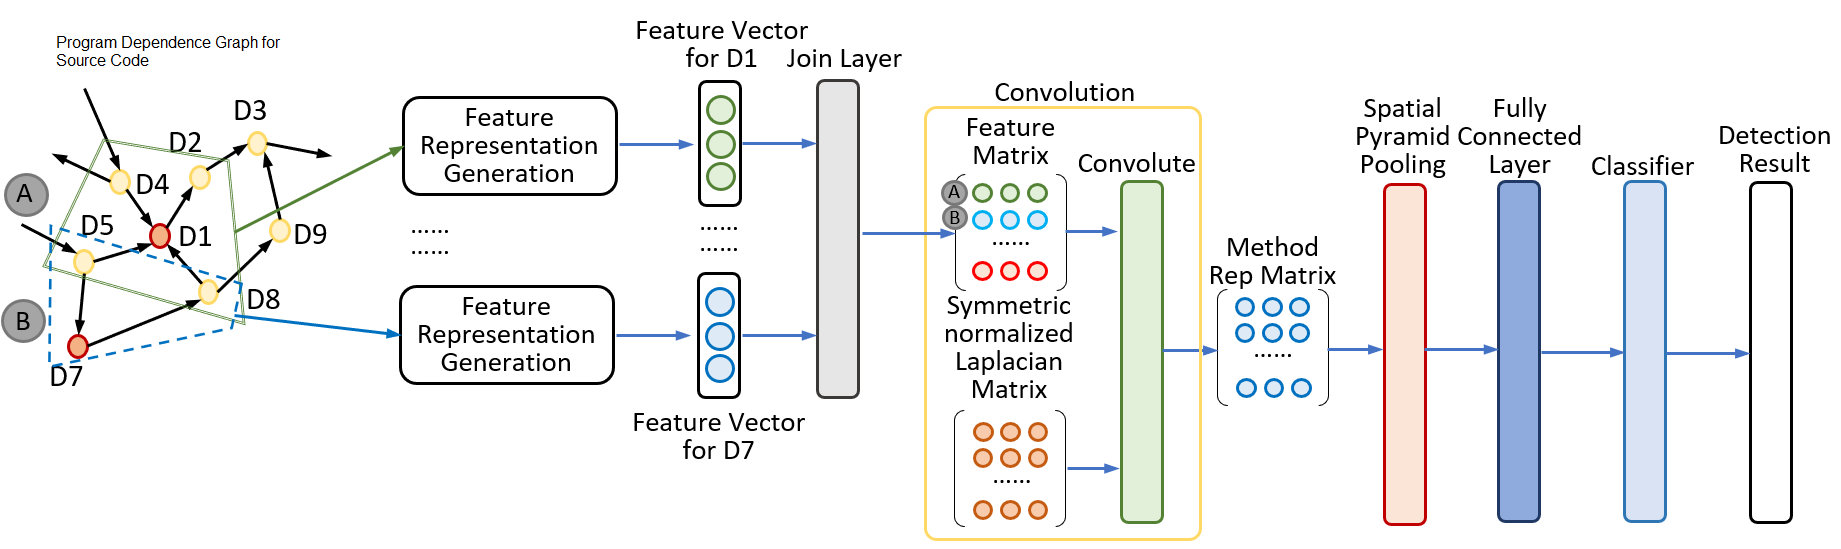
\includegraphics[width=6.5in]{graph-based-CNN.png}
    \caption{Feature-Attention, Graph-based Convolution Network for
      Vulnerability Detection Model}
    \label{fig:detection-model}
\end{figure}

Figure~\ref{fig:detection-model} shows our design of the Graph-based
Convolution Network (GCN) model for {\em proactive vulnerability
  detection at the source code level}. We also plan to use
Feature-Attention to enhance the GCN, and hereafter we will refer to
the model as FA-GCN. First, the source code under investigation will
be parsed and the program dependence graph (PDG) is extracted.  For
example, in Figure~\ref{fig:detection-model}, D1-D9 represent the
statements in a program under investigation. The edges represent the
control and data dependencies among the statements. For each
statement, we can use any set of features/attributes that are
important to the statements.
%Each node can be associated with attributes.

%devices in an IoT system are modeled as the nodes in a graph structure
%in a GCN. D1-D9 in Figure~\ref{fig:detection-model} are nine example
%IoT devices under study in the system, where the attributes and
%features of a node represent the properties associated with the IoT
%devices.

Similar to CNN using the filter on an image, FA-GCN performs sliding a
small window along all nodes (statements) of the PDG. For example, in
Figure~\ref{fig:detection-model}, the window marked with \circled{A}
for the node $D1$ consists of itself and the neighboring
statements/nodes $D2$, $D4$, $D5$, and $D8$. Another window (marked
with \circled{B}) is for the node $D7$ at the center, including itself
and the neighboring nodes: $D5$ and $D8$. For each window, FA-GCN
generates the feature representation matrix for the statement at the
center. For example, for the window centered at $D1$, it generates the
feature vector $F_{D1}$ for the statement $D1$. 

From the representation vectors for all statements, FA-GCN uses a join
layer to link all these vectors into the Feature Matrix
$\mathcal{F}_{m}$ for method $M$. A row in $\mathcal{F}_m$ corresponds
to a window in the input PDG graph.  Next, FA-GCN performs the
convolution operation by first calculating the symmetric normalized
Laplacian matrix~$\tilde{A}$~\cite{GCN16}, and then calculating the
convolution to generate the representation matrix $M_{m}$ for the
subset $S$ of the source code under investigation. After that, we use
the traditional steps as in a CNN model: using a spatial pyramid
pooling layer (to normalize the method representation matrix into a
uniform size, and reduce its total size), and connecting its output to
a fully connected layer to transform the matrix into a vector $V_S$ to
represent the subset $S$ of the IoT devices under study. With $V_S$,
we perform classification by using two hidden layers (controlling the
length of vectors and output) and a softmax function to produce a
prediction score for $S$. We use those scores as {\em vulnerability
  scores to rank the potentially vulnerable code}. The decision for
$m$ as vulnerable or not can be done via a trainable threshold on the
prediction score~\cite{li2018vuldeepecker,li2019improving}. The
detection results in terms of the scores for all statements are
recorded.

%Let us revisit {\em example scenario 1} presented in Section \ref{section:An Example Use Case}, where we assume that IoT devices and computation within them, particularly those that are publicly located within the campus network, can be compromised and used to facilitate other malicious cyber activities. 
% To model this scenario, each node in the FA-GCN model represents an IoT device (e.g., nodes for servers, smartTV, networks, camera, etc.), and the edges represent the interconnections among the devices. To train the FA-GCN, we can use the historical data from the same or similar IoT systems with their devices in the same device category. The data acquisition process is explained in Section~\ref{subsection:Data Acquisition}.

For training, the Vulnerability databases, e.g., Common
Vulnerabilities and Exposures in the National Vulnerability Database
(NVD) can also be used for training the vulnerability detection model.

%\noindent {\bf Risk Scanning Component}. A similar architecture can be used for the risk scanning component in an IoT system. In this case, the input graph is used to represent the connection structures among IoT devices. The attributes of the nodes represent the features and the {\em risk scores for the IoT devices}. To train the model to evaluate the risk scores, we can rely on the historical data of the devices over time. 

\subsection{Explainable AI for Vulnerability Detection}
\label{sec:xai}

\begin{figure}[!hbt]
    \centering
    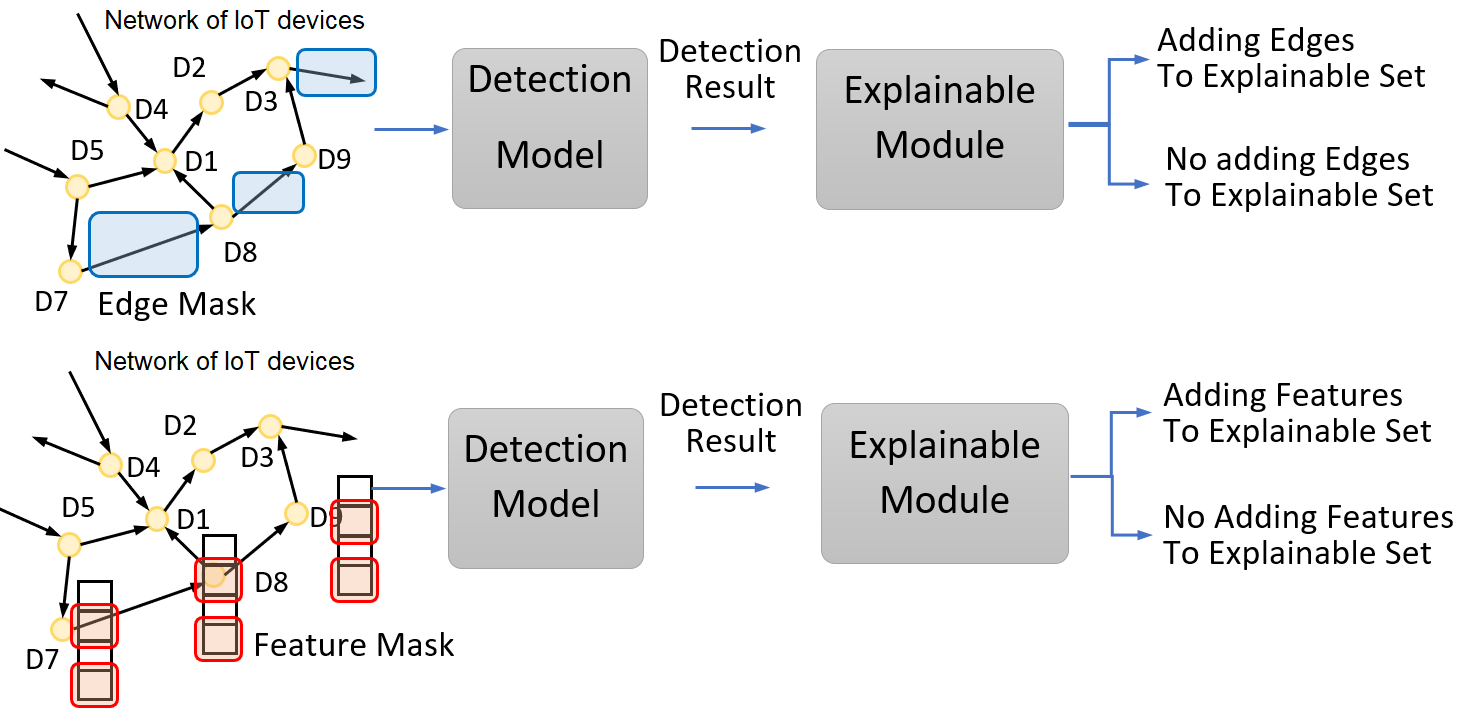
\includegraphics[width=3.8in]{xai-example.png}
    \caption{Graph-based Explainable Model for Vulnerability Detection}
    \label{fig:xai}
\end{figure}

%After each iteration of the detection, it is not necessarily that the detected vulnerable devices at this iteration are  the correct ones. Therefore, we integrate the human expert and analyst in the loop. We then

The explainable AI model takes the detection result with the
vulnerability scores for all the statements and the FA-GCN detection
model itself to produce the {\bf Explainable Set}, {\em which is
  defined as the set containing the parts of the input explaining the
  reason for the model to decide the detected
  vulnerability}. Specifically, it uses both the input graph $G_M$ of
the PDG and the FA-GCN model as the input to obtain the Explainable
Set.
To that end, our goal is to take the FA-GCN and a specific input graph
$G_M$ for PDG of the code under study, and produce the {\em crucial
  sub-graph structures} and {\em crucial features} in $G_M$ that
affect the decision of the FA-GCN detection model.

We leverage our preliminary work on XAI~\cite{fse21-submission}: our
idea is that {\em if removing or altering a node or a feature in the
  input PDG graph of the code does affect much the prediction scores,
  the node or the feature is considered as essential and thus must be
  included in the explainable set}. We use
GNNEXplainer~\cite{GNNExplainer} as follows. It searches for a
sub-graph $\mathcal{G}_M$ in $G_M$ that minimizes the difference in
the prediction scores between using the whole graph $G_M$ and the
minimal graph $\mathcal{G}_M$. Without that subgraph $\mathcal{G}_M$
in the input $G_M$, the model would not decide $G_M$ as vulnerable,
thus, $\mathcal{G}_M$ is considered as {\bf crucial PDG sub-graph}
consisting of {\bf crucial features} in those statements and
connections {\bf relevant to the detected vulnerability}.

\noindent {\em Potential Impacts of Explanations}.  The
statements with crucial features in both Explainable Sets will be
visualized and presented to the security expert. Based on his/her
expertise, (s)he can quickly omit the benign code from the list of
potentially vulnerable code.

%Correctly detected vulnerable device(s) will be isolated and prevented
%from further interaction in the network (i.e., no sending or receiving
%data). The input graph representing the adjusted IoT system with the
%new graph structure of IoT devices will be the input for the next
%iteration of detection.

%Let us revisit {\em example scenario 1} in Section~\ref{section:An Example Use Case} again. Assume that after the first iteration, the model detects that nodes corresponding to servers A, B, and C, router D,  camera E, and  smart TV F are vulnerable. However, with the expertise and knowledge from the expert, router D, which cannot be accessed from the outside, can be quickly eliminated from the suspicious list. The model in the next iteration will not consider router D in the detection process and its parameters will be updated accordingly. The process will continue with the integration of human experts in the loop.
   

\noindent \underline{\bf Formulation.}  Let us formulate how we build
the explainable sets and features/attributes. The input includes the
trained FA-GCN model, the input ($G_M$), and the detection scores for
all the nodes. Figure~\ref{fig:xai} illustrates our
algorithm to train the model.

To derive the explainable sets, the key goal is to find a sub-graph
$\mathcal{G}_M$ in the input $G_M$ that minimizes the
difference in the prediction scores between using the entire graph
$G_M$ and using the minimal graph $\mathcal{G}_M$. To do so, we use
GNNExplainer's {\em masking technique}~\cite{GNNExplainer},
which treats the searching for the minimal graph $\mathcal{G}_M$ as a
learning problem of the {\em edge-mask} set $EM$ of the edges,
and the {\em feature-mask} set $XM$ of the features.
The idea is that learning these two sets $EM$ and $XM$
helps {\tool} derive the explainable sub-graph $\mathcal{G}_M$
and the set of crucial feature $\mathcal{X}_M$
by masking-out the edges in $EM$
and the feature in~$XM$ from $G_M$ (input graph) and $F_M$ (input feature)
({\em Note}: ``masked-out'' is denoted by $\bigodot$):
\begin{equation}\label{eq:11}
\mathcal{G}_M = G_M \bigodot EM
\end{equation}
\begin{equation}
\mathcal{F}_M = F_M \bigodot XM
\end{equation}
In Figure~\ref{fig:xai}, the explainable module checks if the FA-GCN model produces the same result (in this case the result is
vulnerable). If yes, the edge in the edge-mask is not important and
is not included in $\mathcal{G}_M$. Otherwise, the edge is important
and included in $\mathcal{G}_M$.
Similar treatment is for {\em feature-mask} $XM$. In
Figure~\ref{fig:xai}, $FM$ masks the second and fourth features for
each node (IoT device) (Each device has the same number of
features).
Because the numbers of possible sub-graphs and the edge-mask sets
and feature-mask
are untractable, GNNExplainer uses a learning approach for the
edge-mask $EM$ and feature mask $XM$.

Let us formally explain how it works. It
formulates the problem by maximizing the mutual information (MI)
between the minimal graph $\mathcal{G}_M$ and the input~$G_M$:
\begin{equation}\label{maineq}
\max_{\mathcal{G}_M} MI(Y,\mathcal{G}_M, \mathcal{X}_M) = H(Y) - H(Y|G=\mathcal{G}_M, F=\mathcal{X}_M)
\end{equation}
$Y$ is the outcome decision by the FA-GCN model. Thus, the entropy term
$H(Y)$ is constant for the trained FA-GCN model. Maximizing the $MI$
value for all $\mathcal{G}_M$ and $\mathcal{X}_M$ is equivalent to minimizing conditional
entropy $H(Y|G=\mathcal{G}_M, X|F=\mathcal{X}_M)$, which by definition of
conditional entropy can be expressed~as
\begin{equation}
  \label{eq2}
-\mathbb{E}_{Y|\mathcal{G}_M}
  [log P_{FA-GCN} (Y|G=\mathcal{G}_M,F=\mathcal{X}_M)
  \end{equation}
The meaning of this conditional entropy formula is a measure of how
much uncertainty remains about the outcome $Y$ when we know
$G=\mathcal{G}_M$ and $F=\mathcal{X}_M$. GNNEXplainer also limits the
size of $\mathcal{G}_M$ by $K_M$, i.e., taking $K_M$ edges that give
the highest mutual information with the prediction outcome $Y$.
%
Direct optimization of the formula~\ref{eq2} is not tractable, thus,
we can treat $\mathcal{G}_M$ as a random graph variable
$\mathcal{G}$. The objective in Equation~\ref{eq2} becomes:
\begin{equation}
  \label{eq3}
  \min_{\mathcal{G}} \mathbb{E}_{\mathcal{G}_M \sim \mathcal{G}} H(Y|G=\mathcal{G}_M,F=\mathcal{X}_M)
\end{equation}
\begin{equation}
  \label{eq4}
  \min_{\mathcal{G}} H(Y| G=\mathbb{E}_{\mathcal{G}}[\mathcal{G}_M], F = \mathbb{E}_{\mathcal{X}}[\mathcal{X}_M])
\end{equation}
From Equation~\ref{eq3}, we obtain Equation~\ref{eq4} with Jensen's
inequality.  The conditional entropy in Equation~\ref{eq4} can be
optimized by replacing $\mathbb{E}_{\mathcal{G}}[\mathcal{G}_M]$ to be
optimized by masking with $EM$ on the input graph $G_M$.
Now, we can reduce the problem to learning the mask $EM$.
Similar treatment is applied to $XM$.
Details on training can be found in~\cite{GNNExplainer}. The resulting
sub-graph $\mathcal{G}_M$ is directly used as an explainable set. The resulting sub-set of feature $\mathcal{X}_M$ is also an explainable set.

The philosophy is to use Artificial Intelligence (AI) to detect the vulnerability, while using
Intelligence Assistant (IA) by providing explanations for
to support developers in further investigation.
